\section{Kopplingsschema}

\vspace{-20pt}
Robotens elektronik är uppdelad på två virkort. Därför presenteras här ett kopplingsschema för varje virkort.

\vspace{-20pt}
\subsection{Sensorenhet}
\nyBild{sensor.png}{Kopplingsschema för virkortet som innehåller sensorenheten.}{senskoppling}{1}

\textbf{Komponentförteckning}
\vspace{-10pt}
\begin{packed_enumerate}
\item[1.] Sensorenhetens processor, ATmega1284P
\item[2 \& 3.] 16-kanals multiplexer för linjesensor, HEF4067B
\item[4.] Reflexsensormodul
\item[5 \& 6.] Kontakt för kabel till avståndssensor för sidoskanner, GP2D120
\item[7 \& 8.] Kontakt för kabel till servo för sidoskanner, HS-422
\item[9.] Kontakt för JTAG-kabel
\item[10.] Klockgenerator, EXO-3 20 MHz
\item[11 \& 14.] Resistor för lågpassfilter, 18 k$\Omega$
\item[12 \& 13.] Kondensator för lågpassfilter, 100 nF
\item[15.] Kondensator för reset av Sensorenhet, 4700 nF
\item[16.] Resetknapp för Sensorenhet
\item[17.] Pullup-resistor för reset av Sensorenhet
\item[18.] Kontakt för kabel till RFID-läsare, Parallax Serial Reader
\end{packed_enumerate}

\subsection{Kommunikationsenhet, Armenhet, Chassienhet}
\begin{figure}[H]
\centering
 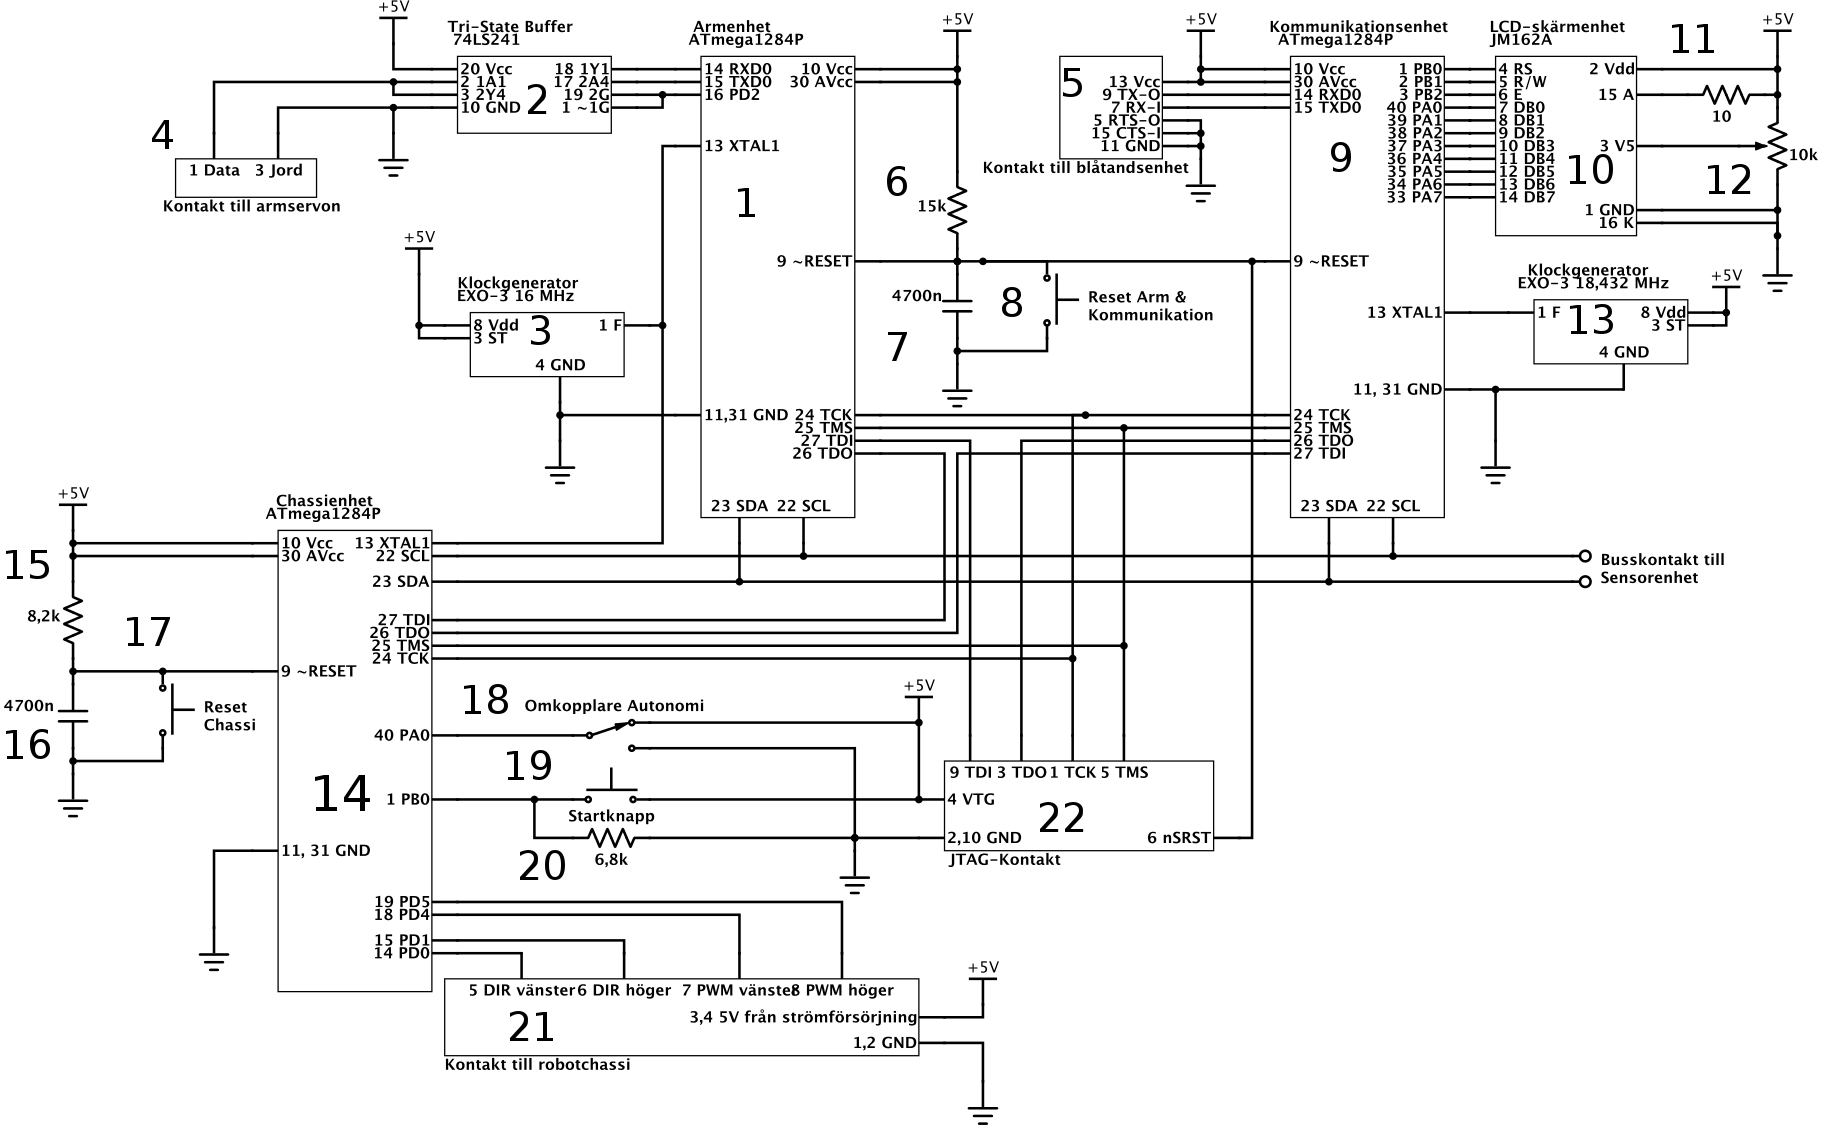
\includegraphics[angle=90,width=0.85\textwidth]{bilder/chassiarmkomm.png}
  \emph{\caption{Kopplingsschema över virkortet som innehåller kommunikationsenheten, chassienheten och armenheten.} \label{fig:chassiarmkomm}}
  
\end{figure}

\textbf{Komponentförteckning}
\begin{packed_enumerate}
\item[1.] Processor Armenhet, ATmega 1284P
\item[2.] Tri-state buffer, 74LS241
\item[3.] Klockgenerator för Armenhet och Chassienhet, EXO-3 16 MHz  
\item[4.] Kontakt för kabel till armservon
\item[5.] Kontakt för kabel till blåtandsenhet
\item[6.] Pullup-resistor för reset av Kommunikationsenhet och Armenhet, 15 k$\Omega$
\item[7.] Kondensator för reset av Kommunikationsenhet och Armenhet, 4700 nF
\item[8.] Resetknapp för Kommunikationsenhet och Armenhet
\item[9.] Processor Kommunikationsenhet, ATmega 1284P
\item[10.] Skärmenhet för LCD-skärm, JM162A
\item[11.] Resistor för att begränsa strömmen till LCD-skärmens bakgrundsbelysning, 10 $\Omega$
\item[12.] Potentiometer för att justera LCD-skärmens kontrast, 0 - 10 k$\Omega$
\item[13.] Klockgenerator för Kommunikationsenhet, EXO-3 18.432 MHz
\item[14.] Processor för Chassienhet, ATmega 1284P
\item[15.] Pullup-resistor för reset av Chassienhet, 8,2 k$\Omega$
\item[16.] Kondensator för reset av Chassienhet, 4700 nF
\item[17.] Resetknapp för Chassienhet
\item[18.] Omkopplare för att växla mellan autonomt och fjärrstyrt läge
\item[19.] Startknapp för att påbörja autonom drift
\item[20.] Pulldown-resistor för startknappen
\item[21.] Kontakt för kabel till robotchassi, tillför spänning +5 V till virkortet
\item[22.] Kontakt för JTAG-kabel.
\end{packed_enumerate}


\section{Utdrag från programlistning}
Utdrag ur programkod från tre filer, dessa är inte kompletta utan endast utdrag för att exemplifiera kodstruktur.

\begin{listing}{1}
/**
 *	@file bus.c
 *	@author Andreas Runfalk & Patrik Nyberg
 *
 *	Functions for intra processor communication over the two wire
 interface
 */

#include <avr/io.h>
#include <avr/interrupt.h>

/**
 *	Temporary storage for received data
 */
uint16_t bus_data;

/**
 *	Temporary storage for response data
 */
uint16_t bus_response_data;

/**
 *	Array of response callbacks used by bus_register_response()
 and bus_call_response()
 */
uint16_t (*response_callbacks[64])(uint8_t, uint16_t) = {0};

/**
 *	Array of receive callbacks used by bus_register_receive() and
 bus_call_receive()
 */
void (*receive_callbacks[64])(uint8_t, uint16_t) = {0};

/**
 *	Start listening on given address and enable interrupts
 *
 *	@param address 7-bit address to listen to
 */
void bus_init(uint8_t address) {
	// Bus speed, approximately 70 kHz
	TWBR = 0x80;

	// Enable internal pull-up for SDA and SCL
	PORTC |= 0x03;

	// Set address on bus
	TWAR = (address << 1) | 1;

	// Enable the bus
	TWSR &= 0xfc;
	TWCR = (1 << TWEN) | (1 << TWEA) | (1 << TWIE);

	sei();
}

/**
 *	Try to acquire control over the bus. Will continuously retry
 until control is
 *	aquired. Possible status codes are:
 *
 *	- 0 if bytes were successfully sent
 *
 *	@return Status code
 */
uint8_t bus_start(void) {
	uint8_t status_code;
	cli();
	TWCR = (1 << TWINT) | (1 << TWSTA) | (1 << TWEN) | (1 << TWIE)
		| (1 << TWEA);

	// Wait for TWINT to go high
	while (!(TWCR & (1 << TWINT)));

	status_code = TWSR & 0xf8;
	sei();

	// Check if failure to seize bus
	switch (status_code) {
		case 0x08: // Start
		case 0x10: // Repeated start
			return 0;
		case 0x00:
			cli();
			TWCR &= 0xff ^ (1 << TWSTA);
			TWCR |= (1 << TWINT) | (1 << TWSTO);
			while (!(TWCR & (1 << TWINT)));
			sei();
		case 0xf8:
		default:
			// Catastrophic failure, retry
			return bus_start();
	}
}

/**
 *	Let go of the control over the buss
 */
void bus_stop(void) {
	TWCR |= (1 << TWINT) | (1 << TWSTO) | (1 << TWEA);
}

/**
 *	Write a byte of data on the bus
 *
 *	@param data Data byte to write
 *
 *	@return Masked status code from TWSR
 */
uint8_t bus_write(uint8_t data) {
	uint8_t status_code;

	cli();
	TWDR = data;
	TWCR &= 0xff ^ (1 << TWSTA) ^ (1 << TWSTO);
	TWCR |= (1 << TWINT) | (1 << TWEN) | (1 << TWEA);

	// Wait for TWINT to go high (package sent)
	while (!(TWCR & (1 << TWINT)));

	status_code = TWSR & 0xf8;
	sei();

	return status_code;
}
\end{listing}
\begin{listing}{1}
/**
 *	@file automatic_steering.c
 *	@author Lucas Nilsson
 *
 *	Calculates steering direction based on current robot position
 */

#include "automatic_steering.h"

/**
 *	Store previous error as set by pd_update()
 */
int8_t prev_error;

/**
 *	Bus callback for setting proportional gain in PD controller
 *
 *	@param id Unused
 *	@param kp_data Proportional gain to use
 */
void engine_set_kp(uint8_t id, uint16_t kp_data)
{
	proportional_gain = kp_data;
}

/**
 *	Bus callback for setting proportional gain in PD controller
 *
 *	@param id Unused
 *	@param kd_data Derivative gain to use
 */
void engine_set_kd(uint8_t id, uint16_t kd_data)
{
	derivative_gain = kd_data;
}

/**
 *	Calculate new steering based on passed current error and
 previous error
 *
 *	@param curr_error
 *
 *	@return Steering wheel position to use. Negative means turn
 left and positive
 *	        turn right.
 */
int16_t pd_update(int8_t curr_error)
{
	double diff;
	int16_t p_term;
	double d_term;

	// differentiation
	diff = curr_error - prev_error;

	// scaling
	p_term = proportional_gain * curr_error;
	d_term = derivative_gain  * diff;

	// save current error as previous error for next iteration
	prev_error = curr_error;

	// Return regulated signal
	return p_term + floor(d_term);
}

/**
 *	Set regulator constants to default values. To be used when
 initializing robot
 */
void regulator_init(void)
{
	prev_error = 0;
	proportional_gain = 180;
	derivative_gain = 5;
}
\end{listing}
\begin{listing}{1}
/**
 *	@file servo.c
 *	@author Andreas Runfalk
 *
 *	Handles tri-state buffer control and basic servo
 communications. Many
 *	functions in this file should only be used in conjunction with
 'macros defined
 *	in servo.h.
 *
 *	This library is not thread safe. No servo communication should
 _ever_ be done in interrupts.
 */

#include "servo.h"
#include "../shared/LCD_interface.h"
#include "../shared/bus.h"

/**
 *	Set tri-state buffer to write mode
 */
void servo_enable_write(void) {
	// Set tri-state buffer to write
	PORTD |= 1 << PORTD2;

	// Wait for tri-state buffer to switch directions
	_delay_us(20);
}

/**
 *	Set tri-state buffer to read mode
 */
void servo_enable_read(void) {
	while (!usart_tx_complete());

	// Set tri-state buffer to read
	PORTD &= ~(1 << PORTD2);

	// Wait for tri-state buffer to switch directions
	_delay_us(20);
}

/**
 *	Initialize USART communication and tri-state buffer control
 */
void servo_init(void) {
	usart_init(SERVO_DEFAULT_BAUD_RATE);

	// Enable control of tri-state buffer and put in read mode
	DDRD |= 1 << DDD2;
	PORTD &= ~(1 << PORTD2);
}

/**
 *	Calculate servo checksum for given array from _first_index_ to
 _last_index_
 *
 *	@param first_index First index of array to include
 *	@param last_index Last index of array to include
 *	@param parameters[] Array to calculate checksum for
 *
 *	@return Checksum
 */
uint8_t servo_calculate_checksum(uint8_t first_index, uint8_t last_index, uint8_t parameters[]) {
	uint8_t i;
	uint8_t checksum = 0;

	for (i = first_index; i <= last_index; i++) {
		checksum += parameters[i];
	}

	return ~checksum;
}

/**
 *	Read response from a servo. Possible status codes are:
 *
 *	- 0 if successful
 *	- 1 if read timed out
 *	- 2 if checksum is wrong
 *	- 3 if incorrect non 0xff start bytes
 *	- 4 if wrong servo return status
 *	- 5 if servo didn't understand the instruction
 *	- 6 if servo max torque can't handle applied load
 *	- 7 if checksum is incorrect
 *	- 8 if sent instruction is out of range
 *	- 9 if servo is overheated
 *	- 10 if goal position is out of limit range
 *	- 11 if input voltage is too low or too high
 *
 *	@param[in] id Servo ID that response is expected from
 *	@param[out] parameters Array that should hold response data.
 *	This must be big enough to fit all returned parameters.
 *       
 *	@return Status code
 */
uint8_t servo_receive(uint8_t id, uint8_t *parameters) {
	uint8_t i;
	uint8_t data[256];
	uint8_t data_length = 0;

	// Fetch bytes into an array of length data_length
	// 0:     Start (0xff)
	// 1:     Start (0xff)
	// 2:     ID of servo
	// 3:     Number of data packets (error code + parameters +
	checksum)
	// 4:     Error code
	// 5-...: Parameters
	// Last:  Checksum
	for (i = 0; data_length == 0 || i < data_length; i++) {
		if (usart_read_byte(&data[i]) != 0) {
			// Read timed out
			return 1;
		}

		// Mark how many bytes to expect and pray that this is not
		wrong
		if (i == 3) {
			data_length = data[i] + 4;
		}
	}

	// Calculate checksum and compare against received one
	if (data[data_length - 1] != servo_calculate_checksum(2,
	data_length - 2, data)) {
		return 2;
	}

	// Verify that start bytes we're correct
	if (data[0] != 0xff || data[1] != 0xff) {
		return 3;
	}

	// Verify that correct servo returned data
	if (data[2] != id) {
		return 4;
	}

	// Check if there was an error code
	if (data[4]) {
		if (data[4] & SERVO_ERROR_INSTRUCTION) {
			return 5;
		} else if (data[4] & SERVO_ERROR_OVERLOAD) {
			return 6;
		} else if (data[4] & SERVO_ERROR_CHECKSUM) {
			return 7;
		} else if (data[4] & SERVO_ERROR_RANGE) {
			return 8;
		} else if (data[4] & SERVO_ERROR_OVERHEAT) {
			return 9;
		} else if (data[4] & SERVO_ERROR_ANGLE_LIMIT) {
			return 10;
		} else if (data[4] & SERVO_ERROR_INPUT_VOLTAGE) {
			return 11;
		}
	}

	// Read parameters into given array if not null pointer
	if (data_length > 5 && parameters != 0) {
		for (i = 5; i < data_length - 1; i++) {
			parameters[i - 5] = data[i];
		}
	}

	return 0;
}
/**
 *	Transfer data to servo. To be used with variable length functions
 *
 *	@param id Servo ID
 *	@param instruction Instruction type
 *	@param data_length Number of parameters in data
 *	@param data Variable argument list of parameters to send as
 obtained by `va_start()`
 */
void vservo_send(
	uint8_t id, uint8_t instruction, uint8_t data_length, va_list
	data)
{
	uint8_t i;

	uint8_t packet_length = data_length + 6;
	uint8_t packet[packet_length];

	packet[0] = 0xff;            // Start byte
	packet[1] = 0xff;            // Start byte
	packet[2] = id;              // Servo ID
	packet[3] = data_length + 2; // Length of data + instruction +
	checksum
	packet[4] = instruction;     // Instruction type (read, write,
	ping)

	for (i = 0; i < data_length; i++) {
		packet[i + 5] = (uint8_t)va_arg(data, int);
	}

	// Add checksum to last byte
	packet[packet_length - 1] = servo_calculate_checksum(
		2, packet_length - 2, packet);

	// Disable interrupts while writing data
	cli();

	// Clear buffer before sending to be sure there is not junk
	usart_clear_buffer();

	servo_enable_write();
	for (i = 0; i < packet_length; i++) {
		usart_write_byte(packet[i]);
	}

	// Indicate that all bytes are sent so servo_enable_read can
	wait for all
	// bytes to be transmitted before changing tri-state buffer
	usart_tx_frame();

	// Enable receiving so interrupts can be handled properly
	servo_enable_read();

	// Re-enable interrupts once write is complete
	sei();
}
\end{listing}

\section{ID:n till buss}
\label{sec:callbacks}
\subsection{Delsystem sensor}

\begin{table}[H]
\centering
\label{tab:callbacks-sensor}
\begin{tabularx}{\textwidth}{|l|l|X|}
\hline
\textbf{ID} & \textbf{Sändning/förfrågan} & \textbf{Funktion [data]} \\ \hline
1 & Oanvänd & \\ \hline
2 & Sändning & Kalibrering av linjesensor \\ \hline
3 & Förfrågan & Linjesensordata \\ \hline
4 & Förfrågan & Tyngdpunkt \\ \hline
5 & Sändning & Sätt tejpreferens [ny tejpreferens] \\ \hline
6 & Oanvänd & \\ \hline
7 & Oanvänd & \\ \hline
8 & Oanvänd & \\ \hline
9 & Sändning & Sätt aktivitet [0 = linjeföljning, 1 = skanna vänster, 2 = skanna höger] \\ \hline
10 & Sändning & Läs RFID-tag \\ \hline
\end{tabularx}
\caption{De funktioner för att reagera på bussöverföringar som sensorenheten har implementerat.}
\end{table}

\subsection{Delsystem chassi}

\begin{table}[H]
\centering

\begin{tabularx}{\textwidth}{|l|l|X|}
\hline
\textbf{ID} & \textbf{Sändning/förfrågan} & \textbf{Funktion [data]} \\ \hline
0 & Sändning & Nödstopp \\ \hline
1 & Oanvänd & \\ \hline
2 & Sändning & Arm klar [0 = plockat up, 1 = lagt ner, 2 = hittade inget] \\ \hline
3 & Sändning & Starta linjeföljning \\ \hline
4 & Sändning & RFID inläst \\ \hline
5 & Oanvänd & \\ \hline
6 & Oanvänd & \\ \hline
7 & Oanvänd & \\ \hline
8 & Sändning & Uppdatera manuell styrning, via CMD\_CHASSI\_MOVEMENT i tabell \ref{tab:commands}\\ \hline
9 & Oanvänd & \\ \hline
10 & Oanvänd & \\ \hline
11 & Sändning & Sätt Kp [nytt värde på Kp] \\ \hline
12 & Sändning & Sätt Kd [nytt värde på Kd] \\ \hline
\end{tabularx}
\caption{De funktioner för att reagera på bussöverföringar som chassienheten har implementerat.}
\label{tab:callbacks-chassi}
\end{table}

\subsection{Delsystem kommunikationsenhet}

\begin{table}[H]
\centering

\begin{tabularx}{\textwidth}{|l|l|X|}
\hline
\textbf{ID} & \textbf{Sändning/förfrågan} & \textbf{Funktion [data]} \\ \hline
1 & Oanvänd & \\ \hline
2 & Sändning & Rad 1 på skärm för sensorenheten \\ \hline
3 & Sändning & Rad 2 på skärm för sensorenheten \\ \hline
4 & Sändning & Rad 1 på skärm för armenheten \\ \hline
5 & Sändning & Rad 2 på skärm för armenheten \\ \hline
6 & Sändning & Rad 1 på skärm för chassienheten \\ \hline
7 & Sändning & Rad 2 på skärm för chassienheten \\ \hline
8 & Sändning & Vidarebefordra beslut från chassi till PC \\ \hline
9 & Sändning & Vidarebefordra RFID-tag till PC\\ \hline
10 & Sändning & Vidarebefordra data från sidoskanner till PC \\ \hline
11 & Sändning & Sätt Kp [nytt värde på Kp] \\ \hline
12 & Sändning & Sätt Kd [nytt värde på Kd] \\ \hline
13 & Sändning & Vidarebefordra kalibreringsvärde till PC \\ \hline
\end{tabularx}
\caption{De funktioner för att reagera på bussöverföringar som kommunikationsenheten har implementerat.}
\label{tab:callbacks-komm}
\end{table}

\subsection{Delsystem arm}

\begin{table}[H]
\centering

\begin{tabularx}{\textwidth}{|l|l|X|}
\hline
\textbf{ID} & \textbf{Sändning/förfrågan} & \textbf{Funktion [data]} \\ \hline
0 & Sändning & Nödstopp \\ \hline
1 & Sändning & Kommando till klo [0 = stäng, 1 = öppna] \\ \hline
2 & Sändning & Signal att roboten står på station [0 = vänster, 1 = höger] \\ \hline
3 & Sändning & Vinkel till upplockning [vinkel] \\ \hline
4 & Sändning & x koordinat till upplockning [x] \\ \hline
5 & Sändning & Plocka upp objekt [0 = inget hittades, 1 = föremål hittat] \\ \hline
6 & Sändning & x position för manuell styrning [x] \\ \hline
7 & Sändning & y position för manuell styrning [y] \\ \hline
8 & Sändning & Vinkel för manuell styrning om positiv [vinkel] \\ \hline
9 & Sändning & Vinkel för manuell styrning om negativ [vinkel] \\ \hline
10 & Sändning & Gå till position satt i manuell styrning \\ \hline
11 & Sändning & Uppdatera manuell styrning, via CMD\_ARM\_MOVE i tabell \ref{tab:commands} \\ \hline
12 & Sändning & Lämna av objekt [0 = vänster, 1 = höger] \\ \hline
\end{tabularx}
\caption{De funktioner för att reagera på bussöverföringar som armenheten har implementerat.}
\label{tab:callbacks-arm}
\end{table}

\section{Protokoll för blåtand}
\label{sec:blue}
\begin{table}[H]
\begin{tabularx}{\textwidth}{|l|X|X|}
\hline
\textbf{ID-beteckning} & \textbf{Beskrivning} & \textbf{Parametrar} \\ \hline
PKT\_STOP & Indikerar att roboten ska stoppa all rörelse. & Inga \\ \hline
PKT\_ARM\_COMMAND & Kommando till arm. & Kommando (1), argument (2-10) \\ \hline
PKT\_CHASSIS\_COMMAND & Kommando till chassi. & Kommando (1), argument (2-3) \\ \hline
PKT\_CALIBRATION\_COMMAND & Kommando för kalibrering av sensor. & Sensor id (1) \\ \hline
PKT\_LINE\_DATA & Data från linjesensorn. & Individuella sensorer (1-11), flaggor (12), tyngdpunkt (13), styrutslag (14) \\ \hline
PKT\_RANGE\_DATA & Avstånd från sidoskanner. & sida (1), avstånd (2-3) \\ \hline
PKT\_RFID\_DATA & Värde på RFID-tagg & värde (1) \\ \hline
PKT\_CHASSIS\_DECISION & Beslut från chassi. & beslut (1) \\ \hline
PKT\_PACKET\_REQUEST & Förfrågan om paket från dator. & ID på packet (1) \\ \hline
PKT\_SPOOFED\_REQUEST & Simulerad förfrågan över bussen & Adress för enheten som ska ta emot förfrågan (1), ID på funktionen som ska anropas(2), metadata som ska föras med förfrågan (3-4) \\ \hline
PKT\_SPOOFED\_RESPONSE & Svar på simulerad förfrågan. & Data som returneras av förfrågan (1-2) \\ \hline
PKT\_SPOOFED\_TRANSMIT & Simulerad sändning på bussen. & Data som skickas ut på bussen. (1-2) \\ \hline
PKT\_CALIBRATION\_DATA & Värde efter kalibrering. & Värde (1) \\ \hline
PKT\_LINE\_WEIGHT & Tyngdpunkt från linjesensor. & Tyngdpunkt (1) \\ \hline
\end{tabularx}
\caption{De olika pakettyper som kan skickas mellan roboten och PC och vad de innehåller. Parametrarnas ordningsnummer i parameterföljden anges inom parentes i den sista kolumnen.}
\label{tab:packets}
\end{table}

\begin{table}[H]

\begin{tabularx}{\textwidth}{|l|X|X|}
\hline
\textbf{ID-beteckning} & \textbf{Beskrivning} & \textbf{Parametrar} \\ \hline
CMD\_ARM\_MOVE & Arm ska röra sig. & Koordinat (1), riktning (2) \\ \hline
CMD\_ARM\_GRIP & Stäng gripklo. & Inga \\ \hline
CMD\_ARM\_RELEASE & Öppna gripklo. & Inga \\ \hline
CMD\_ARM\_PREDEFINED\_POS & Rör arm till fördefinierad position. & ID på position \\ \hline
CMD\_ARM\_STOP & Stanna alla rörelser. & Inga \\ \hline
CMD\_ARM\_MOVE\_POS & Rör arm till position. & x (1), y (2), vinkel (3) \\ \hline
CMD\_CHASSIS\_START & Starta linjeföljning. & Inga \\ \hline
CMD\_CHASSIS\_STOP & Stoppa linjeföljning & Inga \\ \hline
CMD\_CHASSIS\_PARAMETERS & Sätt nya värde på $K_p$ och $K_d$. & $K_p$(1), $K_d$(2) \\ \hline
CMD\_CHASSIS\_MOVEMENT & Kommando till chassi att ändra sin hastighet eller riktning & Kommando (1) \\ \hline
\end{tabularx}
\caption{De olika undertyper av paket som skickas som kommandon från persondatorgränssnittet till roboten, genom PKT\_ARM\_COMMAND eller PKT\_CHASSIS\_COMMAND. Parametrarnas ordningsnummer i parameterföljden anges inom parentes i den sista kolumnen.}
\label{tab:commands}
\end{table}

\begin{table}[H]
\label{decision}
\begin{tabularx}{\textwidth}{|l|X|}
\hline
\textbf{ID-beteckning} & \textbf{Beskrivning} \\ \hline
DEC\_PICKUP\_RIGHT & Plockar upp föremål höger. \\ \hline
DEC\_PICKUP\_LEFT & Plockar upp föremål vänster. \\ \hline
DEC\_PUT\_DOWN\_RIGHT & Lägger ner föremål höger. \\ \hline
DEC\_PUT\_DOWN\_LEFT & Lägger ner föremål vänster.  \\ \hline
DEC\_NO\_MATCH & RFID var inte korrekt.  \\ \hline
DEC\_STATION\_HANDLED & Station redan behandlad.  \\ \hline
DEC\_NO\_ID\_FOUND & Ingen RFID-tagg hittade på stationen.  \\ \hline
DEC\_ARM\_PICKED\_UP & Arm har plockat upp ett föremål. \\ \hline
DEC\_ARM\_PUT\_DOWN & Arm har lagt ned ett föremål. \\ \hline
DEC\_OBJECT\_NOT\_FOUND & Inget föremål hittades. \\ \hline
DEC\_UNKNOWN\_ERROR & Okänt fel inträffade. \\ \hline
DEC\_ARM\_FAILED & Arm misslyckades med upplockning. \\ \hline
DEC\_START\_LINE & Startade linjeföljning. \\ \hline
\end{tabularx}
\caption{De olika besluten som roboten kan ta och vidarebefordra till persondatorgränssnittet. Dessa skickas som en parameter i PKT\_CHASSIS\_DECISION.}
\end{table}
